% Preamble:
\documentclass{article}

% Packages:
\usepackage{fancyhdr}
\usepackage{amsmath}
\usepackage{graphicx}
\usepackage{tikz}
\usetikzlibrary{arrows}
\usetikzlibrary{backgrounds}

% Title Page Information:
\title{CS23 Assignment Three}
\author{CJ Bridgman-Ford \\ cj.ikaika@gmail.com}
\date{April 4, 2024}

% Make subsections lettered:
\renewcommand{\thesubsection}{\alph{subsection}.}

% fancyhdr Page Styling:
\newcommand{\pagenumber}{\thepage\quad}
\newcommand{\authorname}{CJ Bridgman-Ford}

\pagestyle{fancy}
\renewcommand{\headrulewidth}{0pt}
\fancyhead{}
\fancyfoot[L]{\authorname}
\fancyfoot[C]{}
\fancyfoot[R]{\pagenumber}

% Bigcircled command:

\newcommand\Bigcircled[1]{\raisebox{-0.5mm}{\scalebox{1.7}{$\textcircled{#1}$}}}

% End of Preamble.

% Start of document:
\begin{document}

% Title Page:
\maketitle
\thispagestyle{empty}


\clearpage
% Page 1:
\pagenumbering{arabic}

% Problem 1:
\section{Is $(1, 2, 3, 4) = (1, 2, 4, 3)$?}
\hspace{1cm}\textbf{No.}\textit{ Unlike sets, the order of elements in a tuple matters.}

% Problem 2
\section{Which of the following are equivalent: \\
    $\{a, b, c\}, \{\{a, b\}, c\}, (a, b, c), (a, (b, c)), (b, c, a),
    \\ \{\{a, b, c\}\}, \{b, c, a\}, \{\}, \{\{\}\}$}
\hspace{1cm}\textbf{$\{a, b, c\}$ is equivalent to $\{b, c, a\}$.}\textit{
    All other tuples and sets are inequivalent due to differences in strcture
    or order of elements.}

% Problem 3:

\section{Let $A = \{2, 3, 4\}$ and $B = \{6, 8, 10\}$ and define
    a relation $R$ from $A$ to $B$ as follows:
    For every $(x, y) \in A \times B$, $(x, y) \in R$ means that
    $\frac{y}{x}$ is an integer.}
\subsection{Is $4R6$? Is $4R8$? Is $(3,8) \in R$? Is $(2,10) \in R$?}
\hspace{1cm}\textit{$\frac{6}{4} = 1.5$ is not an integer.}\textbf{ Therefore,
    $4R6$ is not true.}\textit{ $\frac{8}{4} = 2$ is an integer.}\textbf{ Therefore,
    $4R8$ is true.}\textit{ $\frac{8}{3}$ is not an integer.}\textbf{ Therefore,
    $(3,8) \in R$ is not true.}\textit{ $\frac{10}{2} = 5$ is an integer.}
    \textbf{ Therefore, $(2,10) \in R$ is true.}
\subsection{Write $R$ as a set of ordered pairs.}
\hspace{1cm}\textit{$R = \{(2,6),(2,8),(2,10),(3,6),(4,8)\}$.}
\subsection{Write the domain and co-domain of $R$.}
\hspace{1cm}\textit{The domain of $R$ is $A$ and the co-domain is $B$.}
\subsection{Draw an arrow diagram for $R$.}
\begin{center}
    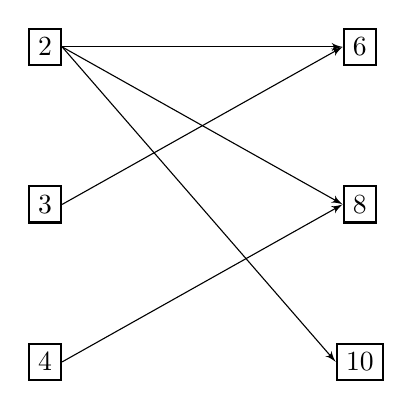
\begin{tikzpicture}
        [
            > = latex', box/.style = {rectangle, draw=black, thick, align=center}
        ]
        \node [box] at (-2, 0)(box2) {2};
        \node [box] at (2, 0) (box6) {6};
        \node [box] at (-2, -2)(box3) {3};
        \node [box] at (2, -2) (box8) {8};
        \node [box] at (-2, -4)(box4) {4};
        \node [box] at (2, -4) (box10) {10};

        \draw[->] (box2.east) -- (box6.west);
        \draw[->] (box2.east) -- (box8.west);
        \draw[->] (box2.east) -- (box10.west);
        \draw[->] (box3.east) -- (box6.west);
        \draw[->] (box4.east) -- (box8.west);
    \end{tikzpicture}
\end{center}
\clearpage

% Problem 4:

\section{Given that $\Omega$ = all students in university, $D$ = day students,
    $M$ = mathematics majors, and $G$ = graduate students, draw a venn diagram for
    this situation and copy it once for each of the given problems. Shade the
    following sets.}
\subsection{Evening and online students:}
\begin{center}
    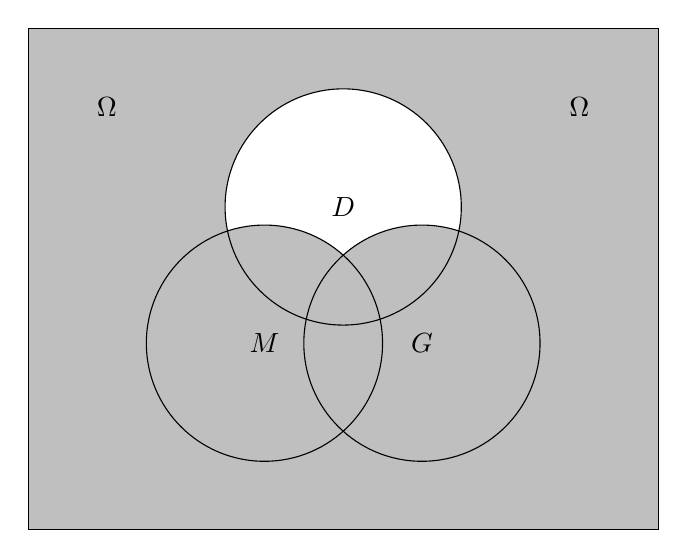
\begin{tikzpicture}
        \fill[gray!50] (-4,-2.37) rectangle (4cm,4cm);
        \fill[white] (0,1.73) circle (1.5cm);
        \fill[gray!50] (1,0) circle (1.5cm);
        \fill[gray!50] (-1,0) circle (1.5cm);
        
        \draw (-4,-2.37) rectangle (4cm,4cm);
        \draw (-1,0) circle (1.5cm);
        \draw (0,1.73) circle (1.5cm);
        \draw (1,0) circle (1.5cm);
        \node at (-3,3) {$\Omega$};
        \node at (3,3) {$\Omega$};
        \node at (0,1.73) {$D$};
        \node at (-1,0) {$M$};
        \node at (1,0) {$G$};
    \end{tikzpicture}
\end{center}
\subsection{Undergraduate mathematics majors:}
\begin{center}
    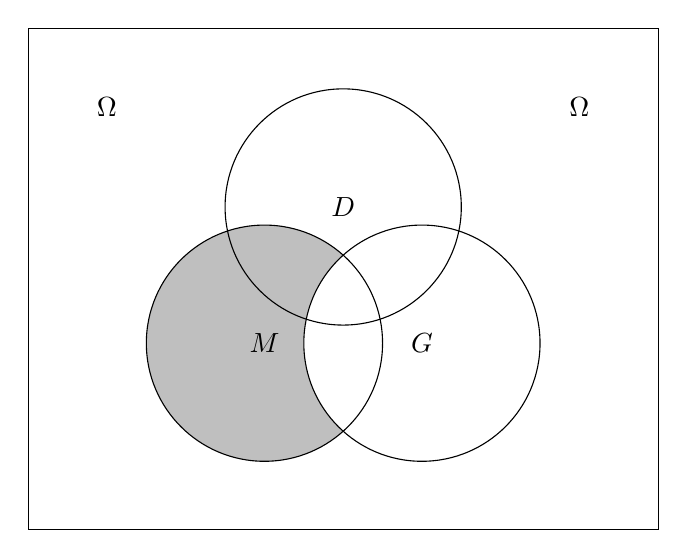
\begin{tikzpicture}
        \fill[gray!50] (-1,0) circle (1.5cm);
        \fill[white] (1,0) circle (1.5cm);
        
        \draw (-4,-2.37) rectangle (4cm,4cm);
        \draw (-1,0) circle (1.5cm);
        \draw (0,1.73) circle (1.5cm);
        \draw (1,0) circle (1.5cm);
        \node at (-3,3) {$\Omega$};
        \node at (3,3) {$\Omega$};
        \node at (0,1.73) {$D$};
        \node at (-1,0) {$M$};
        \node at (1,0) {$G$};
    \end{tikzpicture}
\end{center}
\subsection{Non-math graduate students:}
\begin{center}
    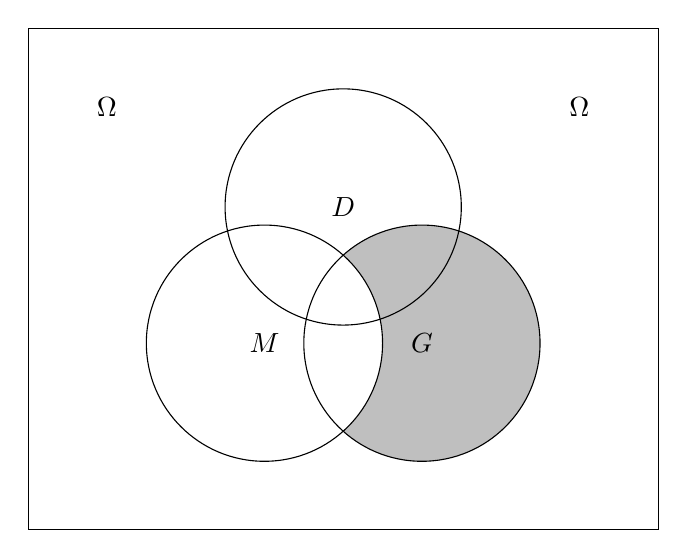
\begin{tikzpicture}
        \fill[gray!50] (1,0) circle (1.5cm);
        \fill[white] (-1,0) circle (1.5cm);
        
        \draw (-4,-2.37) rectangle (4cm,4cm);
        \draw (-1,0) circle (1.5cm);
        \draw (0,1.73) circle (1.5cm);
        \draw (1,0) circle (1.5cm);
        \node at (-3,3) {$\Omega$};
        \node at (3,3) {$\Omega$};
        \node at (0,1.73) {$D$};
        \node at (-1,0) {$M$};
        \node at (1,0) {$G$};
    \end{tikzpicture}
\end{center}
\subsection{Non-math undergraduate students:}
\begin{center}
    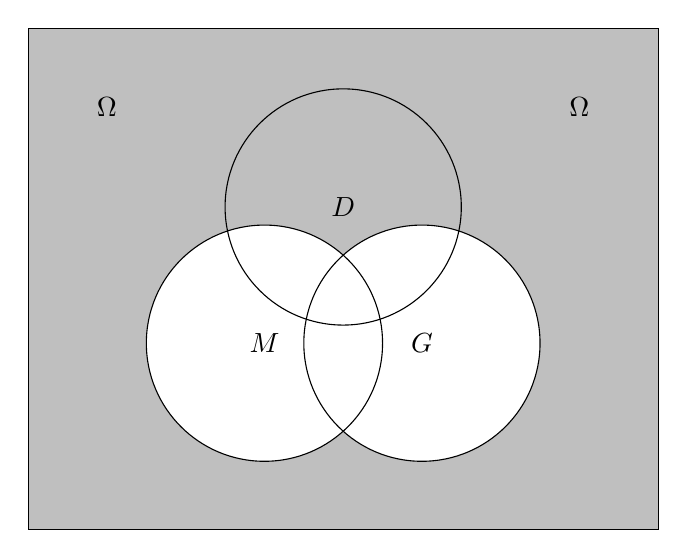
\begin{tikzpicture}
        \fill[gray!50] (-4,-2.37) rectangle (4cm,4cm);
        \fill[white] (1,0) circle (1.5cm);
        \fill[white] (-1,0) circle (1.5cm);
        
        \draw (-4,-2.37) rectangle (4cm,4cm);
        \draw (-1,0) circle (1.5cm);
        \draw (0,1.73) circle (1.5cm);
        \draw (1,0) circle (1.5cm);
        \node at (-3,3) {$\Omega$};
        \node at (3,3) {$\Omega$};
        \node at (0,1.73) {$D$};
        \node at (-1,0) {$M$};
        \node at (1,0) {$G$};
    \end{tikzpicture}
\end{center}

\end{document}